% Compile from docs/ with:
%   pdflatex eeg_mfg_article.tex
%   bibtex eeg_mfg_article
%   pdflatex eeg_mfg_article.tex
%   pdflatex eeg_mfg_article.tex
\documentclass[10pt,journal]{IEEEtran}

\usepackage[T1]{fontenc}
\usepackage[utf8]{inputenc}
\usepackage[english]{babel}
\usepackage{amsmath,amssymb,amsfonts,mathtools}
\usepackage{array}
\usepackage{booktabs}
\usepackage{cite}
\usepackage{graphicx}
\usepackage[hidelinks]{hyperref}
\usepackage{url}

\graphicspath{{../out/article_package/figures/}}

\newcommand{\code}[1]{\texttt{#1}}
\newcommand{\vect}[1]{\mathbf{#1}}

\title{Event-Locked Multi-Feature Directed Dependence in Grasp-and-Lift EEG}

\author{Adrian Przybysz, Bartlomiej Chmiel, and Jarek Duda}

\begin{document}
\maketitle

\begin{abstract}
    We study event-locked scalp EEG from the public Grasp-and-Lift EEG Detection dataset with a multi-feature Granger-style (MFG) lagged-dependence method. The analysis aligns 32-channel recordings to movement phases, applies common-average reference (CAR), maps marginal channel distributions to a common scale, estimates Legendre mixed moments for ordered channel pairs, and summarizes lag profiles with pair-specific PCA. A CAR-only analysis produces many reproducible edges, but most fully stable instances are short-range. We therefore repeat the directed-dependence analysis with 0.5--48 Hz band-pass filtering and a separately fitted PCA basis. Across 27 sensitivity settings, the filtered analysis gives 766 stable edge instances, only five fully stable instances, and two that pass our distance, lag, and asymmetry screen. Both are Fp2--Fp1 edges, so the band-pass result does not support a posterior-to-central cortical connectivity claim. A subject-aware classifier remains a secondary check: the best augmented logistic decoding reaches mean ROC-AUC $0.8698$, while the matched gain over a 500 ms shifted-label control is $+0.0014$. The evidence supports reproducible sensor-level dependence, not anatomical causality.
\end{abstract}

\begin{IEEEkeywords}
    EEG, grasp-and-lift, directed dependence, lagged dependence, Legendre features, PCA, cross-subject meta-analysis, classifier ablation.
\end{IEEEkeywords}

\section{Introduction}
Grasp-and-lift movements unfold through a known sequence of reach, contact, loading, lifting, replacement, and release. This makes the task useful for asking whether delayed dependence between EEG sensors changes with movement phase. Scalar summaries such as Pearson correlation or mutual information reduce each channel pair to one value and may miss concurrent dependence modes at different lags.

We apply a time-delay multi-feature dependence approach inspired by multi-feature correlation analysis~\cite{duda2023timedelay} to the public Grasp-and-Lift EEG Detection dataset derived from WAY-EEG-GAL~\cite{luciw2014wayeeggal,kagglegrasp}. We use MFG as shorthand for a multi-feature Granger-style lagged-dependence estimator: it is directional because the target is represented by an innovation-like signal, but it is not classical VAR Granger causality. For each ordered channel pair and lag, the method estimates a vector of mixed-moment coefficients and uses PCA to extract local variance directions. Because PCA is fitted separately for every ordered pair, identically numbered components across the sensor matrix are not one common physical mode. The output is a set of component-wise sensor maps rather than one global dependence score.

We test which sensor-level dependencies recur across participants, phases, and lags. A classifier ablation assesses MFG-derived information beyond direct EEG features rather than optimizing competition performance~\cite{barachant2015grasp}.

\section{Data}
\subsection{Dataset}
We use the Kaggle \emph{Grasp-and-Lift EEG Detection} release~\cite{kagglegrasp}, based on WAY-EEG-GAL~\cite{luciw2014wayeeggal}. The original experiment contains 12 participants and 3,936 grasp-and-lift trials. Participants reached for an object, grasped it with thumb and index finger, lifted it, held it briefly, replaced it, and released it. Object weight and surface friction varied across trials.

The release contains 96 labelled training series and 24 unlabelled test series. Each labelled series comprises aligned EEG data and frame-wise event labels, whereas the test series contain EEG data without event labels. We use the labelled training data for event-locked cross-subject analysis and held-out classifier validation; the unlabelled test data are not used in the reported analyses.

\subsection{Signals and Labels}
Each EEG series contains 32 scalp channels sampled at 500 Hz. Event annotations contain six binary labels: \code{HandStart}, \code{FirstDigitTouch}, \code{BothStartLoadPhase}, \code{LiftOff}, \code{Replace}, and \code{BothReleased}. The labels are multi-label and frame-wise. Event centers are reconstructed from contiguous positive label blocks and used to build movement phases.

\section{Preprocessing}
Data and event rows are aligned by the shared sample identifier. For each time sample, common-average reference (CAR) is applied across channels:
\begin{equation}
    X_{t,c} \leftarrow X_{t,c} - \frac{1}{C}\sum_{d=1}^{C}X_{t,d},
\end{equation}
where $C=32$ is the number of EEG channels.

The WAY-EEG-GAL/Kaggle release did not apply blink or eye-movement rejection~\cite{luciw2014wayeeggal,kagglegrasp}. We therefore compare CAR-only preprocessing with a repeated directed-dependence analysis using a fresh all-pairs PCA basis after band-pass filtering. Two additional preprocessing operations support sensitivity checks:
\begin{itemize}
    \item \code{bandpass\_0\_5\_48}: fourth-order zero-phase band-pass filtering between 0.5 and 48~Hz;
    \item \code{ocular\_proxy\_regression}: linear regression of every channel on Fp1/Fp2, a lightweight EOG-proxy correction when dedicated EOG channels are unavailable.
\end{itemize}
These options are \emph{not} a substitute for full ICA-based ocular cleaning, but they provide a reproducible way to test whether directed-dependence and classifier findings depend on filtering and frontal eye-proxies. Classifier controls additionally compare \code{all32}, \code{motor\_premotor}, \code{no\_fp1\_fp2}, and \code{ocular\_proxy\_only} channel sets.

\subsection{Event Alignment and Phase Windows}
Event blocks are ordered into grasp cycles. The analysis uses adjacent event phases:
\begin{equation}
    \begin{split}
         & \code{HandStart -> FirstDigitTouch},          \\
         & \code{FirstDigitTouch -> BothStartLoadPhase}, \\
         & \code{BothStartLoadPhase -> LiftOff},         \\
         & \code{LiftOff -> Replace},                    \\
         & \code{Replace -> BothReleased}.
    \end{split}
\end{equation}
For each phase, a fixed two-second EEG window is extracted around the phase center.

\section{Method}
\subsection{Marginal Normalization and MFG Features}
The dependence estimator operates on variables that are approximately uniform on $(0,1)$, separating marginal amplitude distributions from dependence structure. In correlation mode, a channel is standardized to zero mean and unit variance and then mapped through the standard-normal $\mathcal{N}(0,1)$ CDF:
\begin{equation}
    U_t = \Phi\left(\frac{X_t-\mu}{\sigma}\right).
\end{equation}
This z-scoring defines the input to the CDF; it does not assert that the original EEG marginal is Gaussian. In directional mode, the source signal is transformed by an empirical CDF, while the target signal is converted into an innovation-like sequence. The target is predicted from its own past with an AR($p$) model, its residual variance is tracked with an exponential moving average, and the standardized residual is mapped through a Student-$t$ CDF. This follows the moving adaptive Student framework~\cite{duda2023adaptive}, with an important implementation restriction: we fix $\nu=10$ and adapt the residual scale, not the degrees of freedom. The source--target asymmetry is used in the spirit of Granger-style lagged dependence~\cite{granger1980testing}; the resulting directionality is statistical and sensor-level.

\subsection{Legendre Mixed-Moment Features}
For a normalized value $u\in(0,1)$, shifted orthonormal Legendre basis functions are evaluated as
\begin{equation}
    f_k(u)=\sqrt{2k+1}\,P_k(2u-1),\quad k=0,\dots,m,
\end{equation}
where $P_k$ is the Legendre polynomial of degree $k$.

For source channel $i$, target channel $j$, lag $\ell$, and non-constant basis indices $a,b\in\{1,\dots,m\}$, the centered mixed moment is
\begin{equation}
    M_{ijab}(\ell)
    =
    \frac{1}{n_\ell}\sum_{t=1}^{n_\ell}f_a(Y_i(t))f_b(Z_j(t+\ell))
    -
    \bar{f}_{i,a}\bar{f}_{j,b,\ell}.
    \label{eq:mixed_moment}
\end{equation}
Here $Y_i$ denotes the normalized source signal, $Z_j$ denotes the normalized target innovation signal, and $n_\ell$ is the number of valid samples for lag $\ell$. The lag convention is source at time $t$ and target at time $t+\ell$. We use $m=4$, giving $m^2=16$ mixed-moment features per ordered channel pair and lag after removing constant marginal terms.

\subsection{Pair-Specific PCA Dependence Modes}
For each ordered pair $(i,j)$ and lag $\ell$, mixed moments are stacked into a vector $\vect{v}_{ij}(\ell)\in\mathbb{R}^{m^2}$. We fit an all-pairs PCA basis once on the labelled training data, accumulating windows from all phases and selected lags. Each ordered channel pair has its own mean vector and PCA directions. Subject-level phase maps are then projected onto this fixed basis:
\begin{equation}
    s_{ij}^{(r)}(\ell)
    =
    \vect{u}_{ij,r}^{\top}\left(\vect{v}_{ij}(\ell)-\boldsymbol{\mu}_{ij}\right),
\end{equation}
where $\vect{u}_{ij,r}$ is the $r$-th PCA direction and $\boldsymbol{\mu}_{ij}$ is the pair-specific mean vector. PC1--PC3 are ordered by decreasing explained variance separately within each ordered pair. For deterministic orientation, each loading vector was multiplied by $-1$ when its largest-magnitude coordinate was negative. This convention makes the numerical sign reproducible for a fixed fitted basis, but it does not establish a common physiological polarity across ordered sensor pairs. Neither component number nor sign therefore defines a shared physiological coordinate; the reported components are local dependence modes, not anatomical sources.

\section{Meta-Analysis}
The band-pass analysis uses directional mode \code{gc}, lags $0$, $50$, $100$, $150$, and $200$ ms, $m=4$, three PCA components, and 0.5--48 Hz preprocessing. For each subject and each scenario defined by phase, PC, and lag, we retain signed scores but rank directed channel edges by $\lvert s_{ij}^{(r)}(\ell)\rvert$. The cross-subject analysis reads the top $k=10$ edges from each subject-level absolute-score ranking. The sign therefore does not affect an edge's top-$k$ position, and edge selection uses score magnitude rather than a shared positive or negative PCA direction.

Cross-subject reproducibility is quantified by the number of subjects in which an edge appears in the top-$k$ list:
\begin{equation}
    K_{ij}=\#\{\text{subjects where }i\to j\text{ is in top-}k\}.
\end{equation}
With $N=12$ subjects, edge-level significance is evaluated using a one-sided binomial tail:
\begin{equation}
    p=\Pr[X\ge K_{ij}],\quad X\sim\mathrm{Binomial}(N,p_0).
\end{equation}
The null probability is
\begin{equation}
    p_0 = 10\cdot\frac{10}{32(32-1)}=0.100806,
\end{equation}
an inflated top-$k$ chance baseline intended to reduce sensitivity to non-uniform edge-ranking biases. Benjamini--Hochberg FDR correction~\cite{benjamini1995controlling} is applied across tested edges with $\alpha=0.05$. A sensitivity grid over top-$k$, minimum subject count, and $p_0$ inflation is used to identify stable claims.

\subsection{Volume-Conduction Control}
Scalp-level dependence can arise from volume conduction and shared-reference leakage rather than genuine inter-regional coupling. To examine this, each fully stable directed edge is annotated with geodesic inter-electrode distance on a standard 10--20 montage, lag structure, and directional asymmetry (whether the reverse edge is also reproducible). A one-sided permutation test compares the mean edge distance against the mean distance of equally many directed pairs drawn uniformly from the montage. We also apply a conservative screening rule: an edge must be long-range ($>4.5$ cm), non-zero-lag, and directionally asymmetric. Passing this heuristic screen reduces concern about simple adjacency or zero-lag mixing, but it does not remove shared-source, ocular, or reference leakage and does not establish cortical connectivity.

\section{Classifier Validation}
\subsection{Ablation Design}
The classifier tests whether MFG-derived features add predictive information beyond direct EEG time-domain features. It is a secondary check on the directed-dependence representation, not a replacement for the directed-dependence analysis. Three feature sets are compared:
\begin{equation}
    \begin{split}
        \text{baseline} & = \text{direct EEG time-domain features},     \\
        \text{mfg}      & = \text{selected MFG edge-dynamics features}, \\
        \text{combined} & = \text{baseline} + \text{mfg}.
    \end{split}
\end{equation}
Baseline features include standardized EEG samples, temporal differences, lagged samples, rolling means, and rolling RMS windows. The classifier applies band-pass preprocessing to its inputs but uses CAR-only stable-edge selection, whereas the primary inferential analysis uses band-pass-selected edges; it therefore does not validate the band-pass edge set. The controlled results use regularized logistic SGD. The \code{combined} model concatenates baseline and MFG features, whereas score-level fusion averages predictions from separately trained baseline and MFG models.

The primary quantity is
\begin{equation}
    \Delta_{\mathrm{AUC}} =
    \mathrm{ROC\mbox{-}AUC}(\mathrm{augmented})
    -
    \mathrm{ROC\mbox{-}AUC}(\mathrm{baseline}),
\end{equation}
where the augmented model is either the fixed \code{combined} feature set or a fixed fusion setting. When explicitly reported, best augmented denotes the better of these two completed variants for the specified evaluation row. A positive value indicates that MFG-derived information improves held-out sample-level event prediction relative to the direct EEG baseline under the same split and model settings.

\subsection{Controls}
Classifier claims are evaluated with channel-set and timing controls. The channel sets are \code{all32}, \code{motor\_premotor}, \code{no\_fp1\_fp2}, and \code{ocular\_proxy\_only}. The first uses all EEG channels; the second focuses on motor and premotor electrodes; the third removes frontal eye-proxy channels; the fourth is a confound check and is not a target model. Timing controls compare aligned labels with labels shifted by 500 ms. A strong predictive claim requires aligned lift to exceed the matched shifted-label control under the same split and model settings. The stricter participant-specific validation trains and evaluates within held-out series for each subject, then aggregates matched aligned-versus-shifted comparisons across subjects, splits, and hyperparameters.

\section{Results}
\subsection{Representative Dependence Scenarios}
Table~\ref{tab:scenarios} summarizes selected phase/PC/lag scenarios from the evidence tables. All listed scenarios include all 12 subjects. Dominant direction is computed over significant edges and uses anatomical sensor-group names only.

\begin{table*}[t]
    \centering
    \caption{Representative phase/PC/lag scenarios from the meta-analysis.}
    \label{tab:scenarios}
    \scriptsize
    \setlength{\tabcolsep}{3pt}
    \begin{tabular}{@{}p{0.38\textwidth}cccp{0.31\textwidth}@{}}
        \toprule
        Phase                                & PC  & Lag (ms) & Significant edges & Dominant sensor-group direction \\
        \midrule
        \code{LiftOff -> Replace}            & PC1 & 50       & 11    & \code{Parietal -> Parietal} \\
        \code{FirstDigitTouch -> BothStartLoadPhase} & PC2 & 200 & 10 & \code{Frontal -> Parietal} \\
        \code{LiftOff -> Replace}            & PC3 & 50       & 9     & \code{Parietal -> Occipital} \\
        \code{BothStartLoadPhase -> LiftOff} & PC2 & 200      & 8     & \code{Frontal -> Parietal} \\
        \code{BothStartLoadPhase -> LiftOff} & PC1 & 50       & 8     & \code{Parietal -> Parietal} \\
        \bottomrule
    \end{tabular}
\end{table*}

\subsection{Preprocessing Sensitivity}
The CAR-only and band-pass analyses yielded markedly different robustness profiles. In the CAR-only analysis, the sensitivity grid contains 1323 unique stable edge instances and 298 instances remain significant in all 27 grid settings. That raw stability is not enough for a cortical interpretation: 71.1\% of the fully stable CAR-only instances are short-range, and the observed mean inter-electrode distance is only 3.89 cm.

Under band-pass preprocessing, 766 unique edge instances satisfy at least one sensitivity setting, but only five remain significant in all settings. The strongest scenario summaries are dominated by parietal/spatial and frontal-to-parietal directions rather than the predominantly occipital pattern observed with CAR-only preprocessing (Table~\ref{tab:scenarios}). Thus the band-pass analysis yields fewer exactly recurring directed edge instances and does not reproduce the CAR-only posterior-to-central pattern.

\begin{table}[t]
    \centering
    \caption{Directed-dependence summary before and after band-pass preprocessing. The final column counts edges passing the distance/lag/asymmetry screen.}
    \label{tab:preprocess_compare}
    \footnotesize
    \begin{tabular}{lccc}
        \toprule
        Preprocessing & Stable & Fully stable & Screen-passing \\
        \midrule
        CAR-only      & 1323   & 298          & 79        \\
        Band-pass     & 766    & 5            & 2         \\
        \bottomrule
    \end{tabular}
\end{table}

Figure~\ref{fig:dense_modes} provides a representative view of the dense signed scores from the band-pass analysis for \code{FirstDigitTouch -> BothStartLoadPhase}. It displays PC1--PC3 across all five lags before subject-level edge selection. The matrices aggregate accepted phase windows across the labelled recordings and do not encode $K/N$, edge-level significance, or stability. This interval also contains the replicated \code{F7 -> FC5} PC1 edge at 200 ms reported below, but the dense display is not an inferential selection.

\begin{figure*}[t]
    \centering
    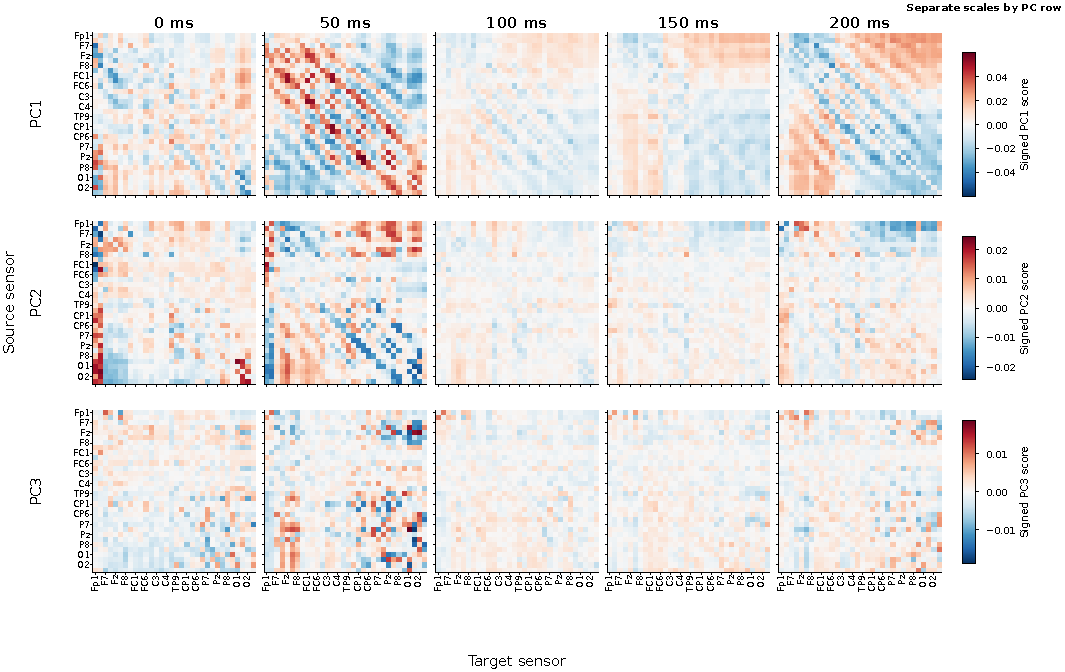
\includegraphics[width=\textwidth]{article_dense_pca_modes_by_lag}
    \caption{Dense signed pair-specific PCA score matrices for \code{FirstDigitTouch -> BothStartLoadPhase} after CAR and 0.5--48 Hz band-pass preprocessing. Columns show lags of 0, 50, 100, 150, and 200 ms, and figure rows show PC1--PC3. Within each matrix, rows are source sensors at $t$ and columns target sensors at $t+\ell$. Each PC row uses one symmetric scale across its five lags; because the rows use separate ranges, color magnitudes should not be compared directly between PC rows. The matrices show the full pre-selection score landscape; cross-subject inference uses subject-level top-$k$ recurrence. PCA bases are fitted separately for each ordered sensor pair.}
    \label{fig:dense_modes}
\end{figure*}

The dense maps show distinct distributed structures across pair-specific modes and lags, but substantially fewer individual directed edges satisfy the cross-subject robustness criteria. Dense matrices contain all pairwise scores before edge selection, whereas subject-level inference requires the same ordered pair to recur in top-$k$ rankings and survive the binomial test and BH-FDR correction.

Full stability requires recurrence across the sensitivity grid and subsequent distance, lag, and asymmetry screening. Similar edge magnitudes can produce between-subject rank changes without eliminating the broader dense pattern.

\subsection{Band-Pass Stable Edges}
\begin{figure*}[t]
    \centering
    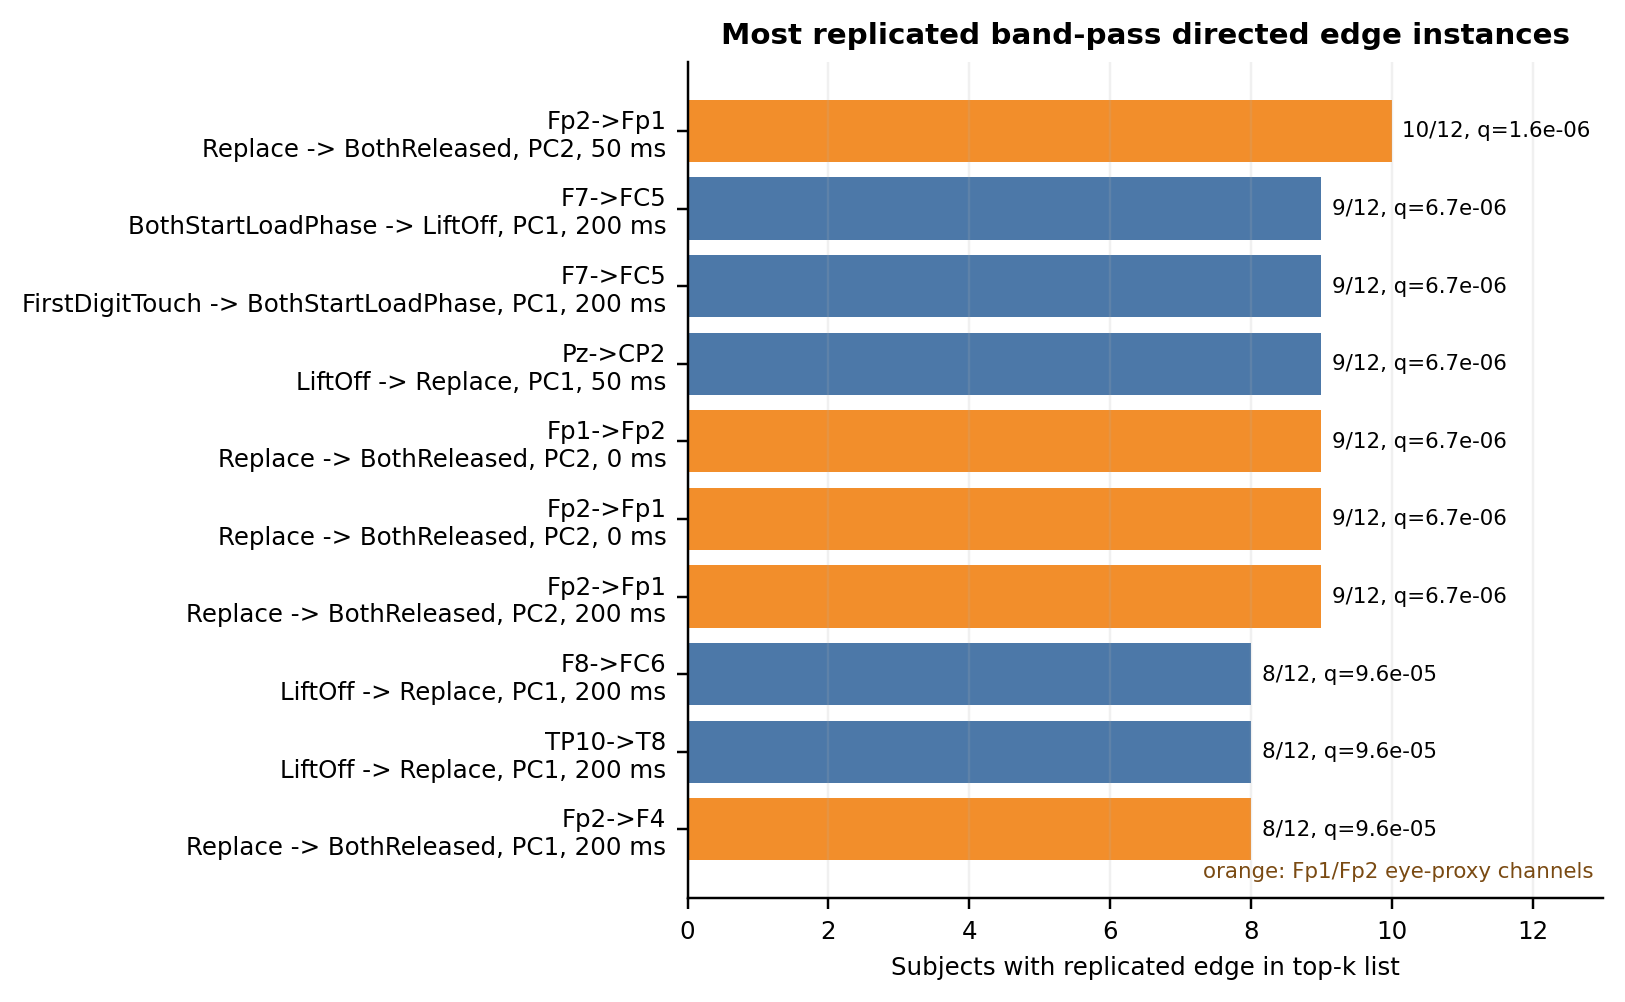
\includegraphics[width=0.86\textwidth]{top_edges_replication.png}
    \caption{Most replicated band-pass directed edge instances. Bar length gives cross-subject recurrence $K/N$, and labels report the BH-FDR-adjusted $q$-value for each phase/PC/lag instance. Orange marks rows involving Fp1/Fp2, interpreted as frontal eye-proxy warnings rather than evidence of cortical connectivity.}
    \label{fig:top_edges}
\end{figure*}

Figure~\ref{fig:top_edges} includes frontal, parietal, and fronto-central pairs rather than the adjacent occipital pairs observed under CAR-only preprocessing. Several strong rows involve Fp1/Fp2, indicating persistent frontal eye-proxy structure after band-pass filtering.

\subsection{Volume-Conduction and Eye-Proxy Control}
Five band-pass instances are fully stable: one is short-range, three occur at non-zero lag, and three are directionally asymmetric. Two pass all three criteria in \code{Replace -> BothReleased}: \code{Fp2 -> Fp1} at 50 ms ($10/12$, $q_{\mathrm{FDR}}=1.56\!\times\!10^{-6}$) and 200 ms ($9/12$, $q_{\mathrm{FDR}}=6.73\!\times\!10^{-6}$). Because~both use frontopolar eye-proxy channels, we treat them as residual ocular/frontal checks rather than anatomical evidence. The band-pass analysis therefore finds reproducible sensor-level dependence but does not support a posterior-to-central cortical connectivity interpretation.

\subsection{Classifier Ablation}
Subject-aware validation provides a secondary test of whether MFG-style edge dynamics add predictive information. The decoder uses three online SGD passes over the participant-specific training files and a fixed sweep over \code{alpha} and fusion weights. Across 288 matched aligned-versus-shifted rows, mean aligned lift is $+0.0026$, mean shifted-control lift is $+0.0012$, and the mean aligned-minus-shifted difference is $+0.0014$. The best timing-control group uses \code{alpha=0.2} and fusion weight $0.25$; its mean baseline AUC is $0.8609$, mean \code{combined} AUC is $0.8616$, mean fusion AUC is $0.8616$, mean best-augmented AUC is $0.8634$, and matched delta is $+0.0020$. The best predictive group uses \code{alpha=0.1} and fusion weight $0.15$: its mean MFG-only AUC is $0.7010$, whereas the mean best-augmented AUC is $0.8698$ with matched delta $+0.0014$. Aggregating deltas by participant gives positive mean delta in 7 of 12 subjects; the subject-level bootstrap 95\% interval for the mean delta is approximately $[0.00001, 0.00283]$, and the one-sided subject sign-test gives $p=0.387$. The classifier therefore provides only modest incremental predictive evidence: MFG-derived edge dynamics add a small amount of controlled information beyond the direct EEG baseline.

\begin{table*}[t]
    \centering
    \caption{Selected classifier validation results. Combined is baseline+MFG feature concatenation, fusion is score-level late fusion, and best aug. is the row-wise better augmented variant.}
    \label{tab:classification}
    \footnotesize
    \begin{tabular}{p{0.30\textwidth}ccccc}
        \toprule
        Setting                             & Baseline & Combined & Fusion & Best aug. & Matched delta \\
        \midrule
        Subject-aware best timing-control group & 0.8609 & 0.8616 & 0.8616 & 0.8634 & +0.0020 \\
        Subject-aware best predictive group     & 0.8674 & 0.8668 & 0.8688 & 0.8698 & +0.0014 \\
        All matched aligned-vs-shifted rows     & --     & --     & --     & --     & +0.0014 \\
        \bottomrule
    \end{tabular}
\end{table*}

\begin{figure*}[t]
    \centering
    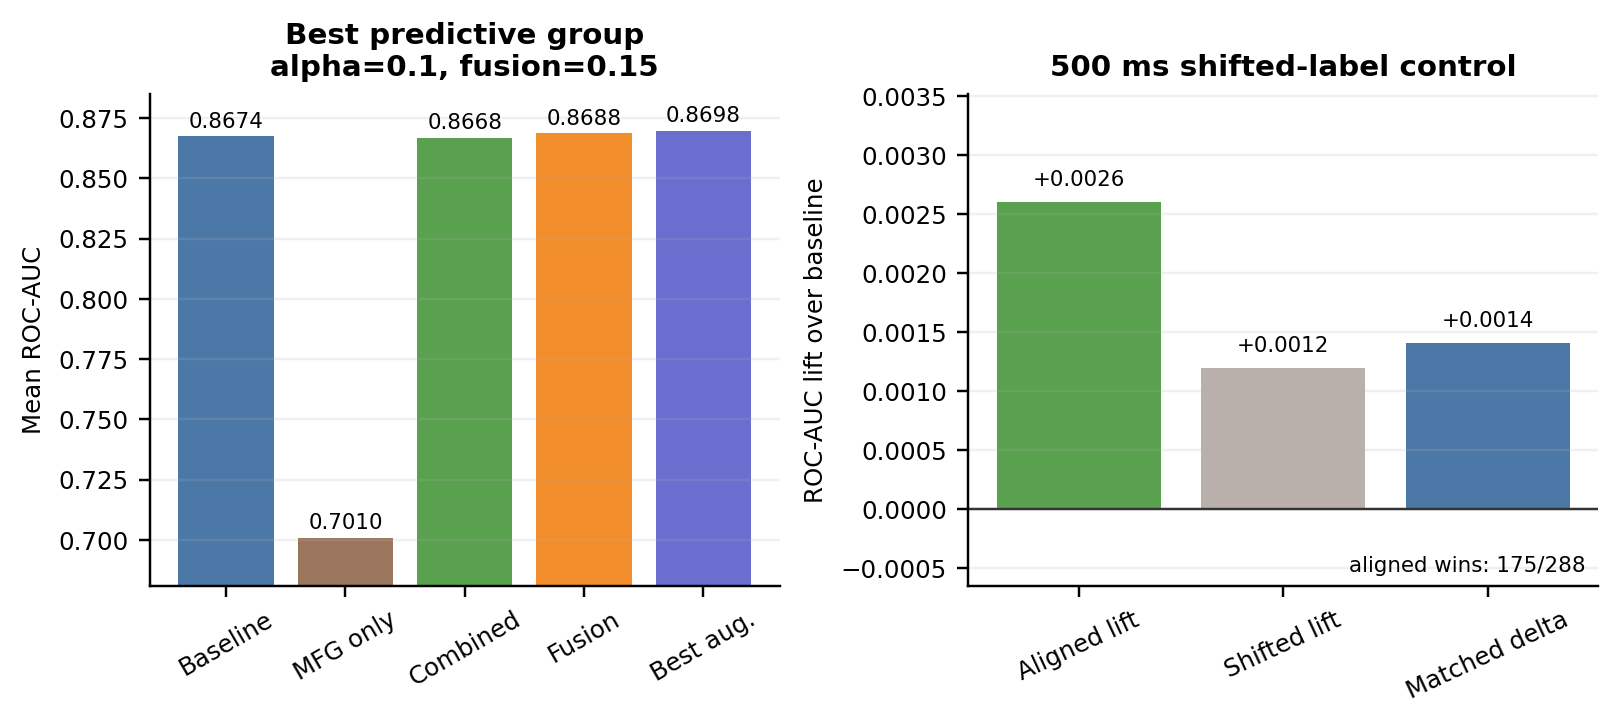
\includegraphics[width=0.86\textwidth]{classification_timing_control.png}
    \caption{Classifier ablation and timing control. In the best predictive group, the relevant comparison is the increment from \code{combined} or fusion over the direct EEG baseline; the MFG-only model is shown for context. The shifted-label panel shows a small positive aligned gain after the 500~ms timing control.}
    \label{fig:classification}
\end{figure*}

\subsection{Timing and Artefact Controls}
Aligned rows exceeded shifted rows in 175 of 288 matched comparisons, although some shifted or artefact-related settings retained positive lift and ocular-proxy-only event-level rows could be large. The timing controls therefore support only a modest predictive contribution from the MFG representation.

\section{Discussion}
The preprocessing variants yielded markedly different robustness profiles. The band-pass analysis shows structured dense score patterns, yet far fewer exact directed edge instances recur across subjects and settings, leaving only two screen-passing Fp2--Fp1 instances. Distributed score structure and stability of a particular ordered pair are different properties. The inferential contrast therefore supports reproducible event-locked sensor dependence but not a strong posterior-to-central cortical connectivity claim.

The classifier ablation tests whether MFG-style edge dynamics help decode events once the direct EEG baseline is already present. It shows a small positive increment. The absolute subject-aware AUC ($\approx 0.87$) is practically useful, but the incremental lift ($\approx +0.002$--$+0.003$) should not be overstated. We therefore treat the classifier as decoder evidence for the representation, not as confirmation of any anatomical connectivity claim.

Unlike competition entries optimized for frame-wise AUC with high-capacity ensembles, extensive feature banks, and stacked prediction layers~\cite{barachant2015grasp}, the classifier here serves only as a secondary validation of the MFG representation. The representation remains traceable to event phase, lag, directed channel pair, and cross-subject replication.

Direction and lag are statistical sensor-level properties rather than anatomical pathways. Source-level interpretation would require source localization, volume-conduction-robust estimators, and independent validation.

\newpage
\section{Limitations}
The analysis has several limitations:
\begin{itemize}
    \item Kaggle labels are frame-wise windows around task events, so event centers are reconstructed from labelled blocks rather than measured directly from the original multimodal event tables.
    \item Only EEG channels from the Kaggle release are used; EMG, kinematic, force, and torque modalities from WAY-EEG-GAL are not included.
    \item The PCA basis and directed-dependence meta-analysis are fitted on the labelled training split, and no independent external cohort is analyzed; the results are exploratory rather than a held-out discovery.
    \item The classifier uses CAR-only stable-edge selection, whereas the primary inferential analysis uses band-pass-selected edges; it therefore does not validate the band-pass edge set.
    \item Scalp-level directed dependence can be affected by volume conduction, reference choice, filtering, shared-source leakage, and ocular contributions. The distance/lag/asymmetry control reduces these concerns but does not remove them.
    \item Pair-specific PCA is variance-driven: high-variance nuisance structure can define a local component even when it is not the dependence direction most relevant to the task. Component labels and signs are not comparable physical coordinates across pairs.
    \item Top-$k$ selection and null inflation are analysis choices. The sensitivity grid checks robustness but does not replace preregistered final parameters.
    \item Classifier evidence is modest in subject-aware validation, and shifted controls also retain small positive lift.
\end{itemize}

\section{Future Work}
Future work should first assess the effects of source mixing and volume conduction. Directed dependence should be recomputed after a surface Laplacian or current-source-density transform, or with volume-conduction-robust estimators such as imaginary coherence or the weighted phase-lag index. This would test whether any robust subset survives under estimators less sensitive to zero-lag field spread.

A full Fp1/Fp2 proxy-regression rerun is also warranted. Participant-level held-out discovery should fit stable edges and PCA bases only on training subjects within each split. Because PCA optimizes variance rather than cross-view association, correlation-oriented approaches such as canonical correlation analysis could be investigated as future alternatives; such approaches are not part of the present analysis. Multimodal WAY-EEG-GAL recordings (EMG, kinematics, force) and an independent EEG grasp dataset would be needed before stronger anatomical or causal language is justified.

\newpage
\section{Conclusion}
We find reproducible event-locked directed lagged dependence in Grasp-and-Lift EEG, while band-pass preprocessing substantially changes the recovered dependence structure. Only five edge instances remain fully stable across the sensitivity grid, and the two that pass the distance/lag/asymmetry screen are Fp2--Fp1 edges. Classifier ablation adds modest evidence that MFG-derived edge dynamics can help held-out event decoding. Taken together, the results support a reproducible sensor-level analysis with a small predictive increment; they do not support an anatomical connectivity claim.

\section{Code Availability}
Code for preprocessing, directed-dependence estimation, cross-subject meta-analysis, classifier validation, and figure generation is available at \url{https://github.com/BartChmiel/mfg-eeg}. A versioned archival release corresponding to the submitted manuscript will be provided before submission.

\newpage
\bibliographystyle{IEEEtran}
\begingroup
\hyphenpenalty=10000
\exhyphenpenalty=10000
\emergencystretch=1em
\bibliography{references}
\endgroup

\end{document}
